\documentclass[conference]{IEEEtran}
\IEEEoverridecommandlockouts
% The preceding line is only needed to identify funding in the first footnote. If that is unneeded, please comment it out.
\usepackage{cite}
\usepackage{amsmath,amssymb,amsfonts,amsthm} % Added amsthm for the proof environment
\usepackage{algorithmic}
\usepackage{algorithm} % Added algorithm for the float and caption
\usepackage{float}
\usepackage{graphicx}
\usepackage{comment}
\usepackage{textcomp}
\usepackage{xcolor}
\usepackage{tikz}
\usetikzlibrary{arrows.meta,positioning,fit,backgrounds,calc,shapes.geometric}
\def\BibTeX{{\rm B\kern-.05em{\sc i\kern-.025em b}\kern-.08em
    T\kern-.1667em\lower.7ex\hbox{E}\kern-.125emX}}

% ---- Palette and node styles shared by every architecture diagram ----
\definecolor{cIn}{HTML}{E8EEF7}
\definecolor{cParse}{HTML}{E4F1E8}
\definecolor{cCore}{HTML}{FBEEDC}
\definecolor{cOut}{HTML}{F2E8F4}
\definecolor{cEval}{HTML}{FAE6E6}
\definecolor{cLine}{HTML}{4A4A4A}
\definecolor{cBand}{HTML}{F7F7F7}

\tikzset{
  blk/.style   = {rectangle, rounded corners=2pt, draw=cLine, line width=0.4pt,
                  align=center, font=\scriptsize, inner sep=3pt,
                  minimum height=8mm, text width=32mm},
  wide/.style  = {blk, text width=42mm},
  slim/.style  = {blk, text width=26mm},
  inb/.style   = {blk, fill=cIn},
  parb/.style  = {blk, fill=cParse},
  corb/.style  = {blk, fill=cCore},
  outb/.style  = {blk, fill=cOut},
  evab/.style  = {blk, fill=cEval},
  band/.style  = {rectangle, rounded corners=3pt, draw=cLine, dashed,
                  line width=0.4pt, inner sep=5pt, fill=cBand},
  bandlab/.style = {font=\scriptsize\bfseries, text=cLine},
  fl/.style    = {-{Latex[length=2mm]}, draw=cLine, line width=0.5pt},
  flb/.style   = {fl, dashed},
  lab/.style   = {font=\tiny, fill=white, inner sep=1pt},
}

\begin{document}

\title{An Architecture for Specification-Driven Test Generation\\and Mutation-Based Evaluation of Platform Software}

\author{
  \IEEEauthorblockN{Areen Vaghasiya}
  \IEEEauthorblockA{\textit{International Institute of Information Technology Bangalore}\\
  Bengaluru, India}
  \and
  \IEEEauthorblockN{Siddharth Palod}
  \IEEEauthorblockA{\textit{International Institute of Information Technology Bangalore}\\
  Bengaluru, India}
  \and
  \IEEEauthorblockN{Akshat Betala}
  \IEEEauthorblockA{\textit{International Institute of Information Technology Bangalore}\\
  Bengaluru, India}
}

\maketitle

\begin{abstract}
Platform software --- libraries and services consumed through an API rather than
through a user interface --- is specified far more often than it is tested against
its specification. We present \textsc{GenATC}, a pipeline that takes three
hand-written artefacts (a JML-style contract, a \emph{test string} naming a
sequence of API calls with concrete inputs, and the library under test) and emits
three executable test artefacts from a single intermediate representation: a
symbolic flavour for Symbolic PathFinder, a runtime-binding JUnit flavour, and a
concrete \emph{singular case} that reports every precondition and postcondition
by name. The architectural contribution is a strict separation between values the
caller invents (\textsc{Client\_Input}) and values the library invents
(\textsc{Server\_Output}); a dedicated propagation scan decides, per call block,
which parameters must be \emph{captured} from an earlier call and \emph{threaded}
forward rather than freshly generated. Because both code flavours are emitted from
one IR, their method signatures and assertions are identical by construction, and
seven cross-example invariants are checked as regression tests over the generated
\emph{code} rather than over its behaviour. We evaluate the generated suites by
mutation: 135 hand-written single-line faults across fourteen libraries are killed
at a rate of 79.3\%, and a generated suite of several hundred operator mutants and
260 machine-generated test strings per library separates the part of that score
owed to the specification from the part owed to the single hand-written sequence.
The per-operator breakdown yields one sharp finding: the pipeline catches faults in
\emph{bookkeeping} almost always and faults in \emph{answers} rarely, and the cause
is a missing quantifier in the specification language rather than a missing test.
\end{abstract}

\begin{IEEEkeywords}
specification-based testing, JML, abstract test cases, symbolic execution, Java
PathFinder, mutation testing, intermediate representation, API sequence testing,
test generation architecture
\end{IEEEkeywords}

\section{Introduction}

A contract for a library operation says what that operation promises \emph{in
isolation}. Real defects in platform software, however, live in \emph{sequences}:
an identifier minted by one call and spent by a later one, a counter that must move
exactly once, a unit of stock that moves from one collaborator to another and is
neither created nor destroyed. Turning a set of per-operation contracts into a test
that exercises such a sequence requires an artefact the contract does not contain
--- an ordering of calls, with concrete values --- and requires the generator to
decide, for every argument of every call, whether the caller supplies it or an
earlier call produced it.

That decision is the pivot of this work. We call a value the caller chooses a
\textsc{Client\_Input} and a value the library invents and returns a
\textsc{Server\_Output}. A \textsc{Client\_Input} can be bound in the test string;
a \textsc{Server\_Output} cannot, because the caller does not know it before the
call. It must instead be captured from the call that produces it and threaded into
every later call that consumes it. Almost every structural feature of the
architecture described here exists to get that distinction right and to keep it
right as the pipeline is extended.

The system takes three hand-written files per library and produces four generated
ones. Nothing about a library is hard-coded in Java: a new library is added by
writing a \texttt{.spec}, a \texttt{.tests} and a \texttt{Helper.java}, and
registering one record in the example driver. Fourteen libraries are carried in the
repository, from a four-line stack to a four-class order service whose
specification is written at a fa\c{c}ade and constrains state owned by three
collaborators it never mentions.

The paper makes three contributions.

\begin{itemize}
\item \textbf{An architecture} (Section~\ref{sec:arch}) in which one intermediate
representation of a test class feeds three code generators, so that two flavours of
the same test --- one for a constraint solver, one for a JUnit runtime --- cannot
disagree about what is being tested.
\item \textbf{A propagation analysis} (Section~\ref{sec:pipeline}) that computes,
block by block, the set of available \textsc{Server\_Output} names and rewrites
helper signatures accordingly, together with seven invariants
(Section~\ref{sec:invariants}) that pin the result and are enforced as tests over
the generated source text.
\item \textbf{A two-sided mutation evaluation} (Section~\ref{sec:eval}): a
hand-written fault set with declared expectations, which behaves as a two-way
regression check on specification quality, beside a mechanically generated suite of
operator mutants and test strings, which measures what the hand-written one can only
assert.
\end{itemize}

\section{Previous Works}

\subsection{Behavioural Interface Specification and JML}

The Java Modeling Language~\cite{b1} attaches \texttt{requires} and \texttt{ensures}
clauses to Java method declarations, with \texttt{\textbackslash old(\textit{e})}
naming a pre-state value and \texttt{\textbackslash result} naming the returned
value. Most JML tooling consumes these clauses as \emph{runtime assertion checks}
compiled into the method under test: the contract is verified wherever the
program happens to call the method. Our use is the dual one. The contract is
consumed as a \emph{generator}: every assertion we emit descends from an
\texttt{ensures} clause and every guard from a \texttt{requires} clause, and the
question of \emph{when} the method is called is answered by a separate artefact,
the test string. We adopt JML's notation for \texttt{\textbackslash old} and
\texttt{\textbackslash result} and add exactly one clause of our own, a
\texttt{state} block, discussed in Section~\ref{sec:lang}.

\subsection{Symbolic Execution and Java PathFinder}

Java PathFinder~\cite{b2} is an explicit-state model checker for Java bytecode;
Symbolic PathFinder~\cite{b3} extends it with a symbolic interpreter and a
constraint solver, so that a method invoked on symbolic inputs yields a set of path
conditions rather than one execution. A test generator that targets SPF must emit
declarations of the form \texttt{Debug.makeSymbolicInteger("x")} and constrain them
with \texttt{Debug.assume}. The awkwardness for sequence testing is that a
\textsc{Server\_Output} is not a free symbolic input: it is whatever the library
returned. Section~\ref{sec:pipeline} describes the design decision that reconciles
the two --- the value is a real formal parameter of the helper method, which the
symbolic flavour re-binds symbolically in its body while the JUnit flavour uses the
argument it was given.

\subsection{Mutation Testing}

Mutation testing~\cite{b4} seeds small syntactic faults into a program and measures
how many a test suite rejects, on the grounds that a suite blind to a deliberate
fault is unlikely to catch an accidental one. The classical Mothra operator set
gives names to the kinds of fault --- arithmetic operator replacement, relational
operator replacement, statement deletion, and so on --- and the survey of
Jia and Harman~\cite{b5} catalogues its development, including the two limitations
that matter here: equivalent mutants, which no suite can kill and which therefore
depress any generated score by an unmeasurable amount, and the cost of re-running
a suite per mutant. We use mutation not to grade a test suite written by hand but
to grade a \emph{specification}: since the suite is generated from the contract,
a surviving mutant is a statement about what the contract fails to say.

\section{System Architecture}
\label{sec:arch}

\subsection{Design Goals}

Four goals shape the structure, and each is visible as a specific boundary in
Fig.~\ref{fig:pipeline}.

\textbf{G1 --- one model, many emissions.} A test is built once as an in-memory
model and printed three times. Two printings that share a model cannot drift apart.

\textbf{G2 --- fail before generating.} Every property of a test string that can be
decided by reading it --- an unknown operation, an unbound argument, an attempt to
bind a \textsc{Server\_Output} --- is decided before a single line of Java is
emitted, so the error message names the input file rather than a compiler
diagnostic on generated code.

\textbf{G3 --- the library is never read.} The generator reads the specification and
the test string only. The library under test is required to satisfy a naming
convention (static state fields matching the \texttt{state} block, one static method
per \texttt{spec}, and \texttt{reset()}), which is what allows the same generated
code to be run against a deliberately broken copy of the library without
regenerating anything about the fault.

\textbf{G4 --- regeneration, not caching.} Every evaluation run re-executes the
whole pipeline from the specification text forward. What is measured is therefore
the pipeline, not a stored artefact.

\begin{figure*}[htbp]
    \centering
    \resizebox{\linewidth}{!}{%
    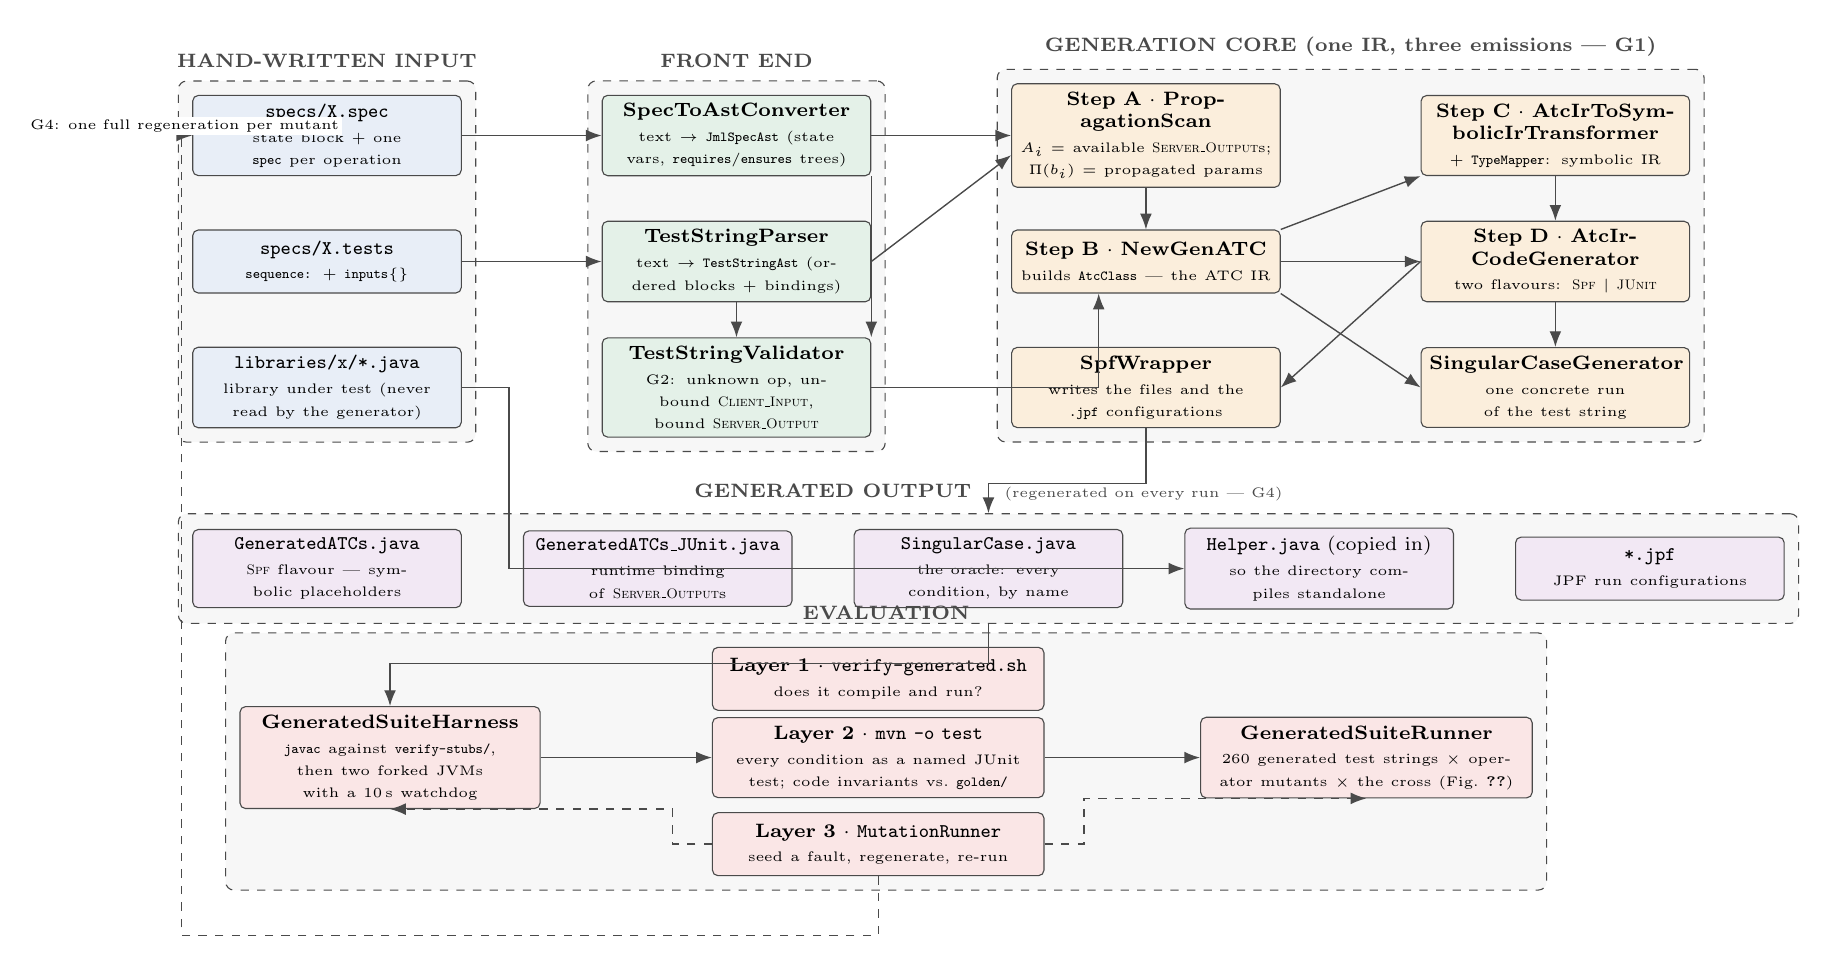
\begin{tikzpicture}
      % ---- INPUT ----
      \node[inb]  (spec)  at (2.4,8.6) {\texttt{specs/X.spec}\\[1pt]\tiny state block + one \texttt{spec} per operation};
      \node[inb]  (tst)   at (2.4,7.0) {\texttt{specs/X.tests}\\[1pt]\tiny \texttt{sequence:} + \texttt{inputs\{\}}};
      \node[inb]  (lib)   at (2.4,5.4) {\texttt{libraries/x/*.java}\\[1pt]\tiny library under test (never read by the generator)};
      \begin{scope}[on background layer]
        \node[band, fit=(spec)(tst)(lib)] (binp) {};
      \end{scope}
      \node[bandlab, above=1pt of binp] {HAND-WRITTEN INPUT};

      % ---- FRONT END ----
      \node[parb] (p1) at (7.6,8.6) {\textbf{SpecToAstConverter}\\[1pt]\tiny text $\rightarrow$ \texttt{JmlSpecAst} (state vars, \texttt{requires}/\texttt{ensures} trees)};
      \node[parb] (p2) at (7.6,7.0) {\textbf{TestStringParser}\\[1pt]\tiny text $\rightarrow$ \texttt{TestStringAst} (ordered blocks + bindings)};
      \node[parb] (val) at (7.6,5.4) {\textbf{TestStringValidator}\\[1pt]\tiny G2: unknown op, unbound \textsc{Client\_Input}, bound \textsc{Server\_Output}};
      \begin{scope}[on background layer]
        \node[band, fit=(p1)(p2)(val)] (bpar) {};
      \end{scope}
      \node[bandlab, above=1pt of bpar] {FRONT END};

      % ---- CORE ----
      \node[corb] (sa) at (12.8,8.6) {\textbf{Step A $\cdot$ PropagationScan}\\[1pt]\tiny $A_i$ = available \textsc{Server\_Output}s; $\Pi(b_i)$ = propagated params};
      \node[corb] (sb) at (12.8,7.0) {\textbf{Step B $\cdot$ NewGenATC}\\[1pt]\tiny builds \texttt{AtcClass} --- the ATC IR};
      \node[corb] (sc) at (18.0,8.6) {\textbf{Step C $\cdot$ AtcIrToSymbolicIrTransformer}\\[1pt]\tiny + \texttt{TypeMapper}: symbolic IR};
      \node[corb] (sd) at (18.0,7.0) {\textbf{Step D $\cdot$ AtcIrCodeGenerator}\\[1pt]\tiny two flavours: \textsc{Spf} $\mid$ \textsc{JUnit}};
      \node[corb] (sg) at (18.0,5.4) {\textbf{SingularCaseGenerator}\\[1pt]\tiny one concrete run of the test string};
      \node[corb] (sw) at (12.8,5.4) {\textbf{SpfWrapper}\\[1pt]\tiny writes the files and the \texttt{.jpf} configurations};
      \begin{scope}[on background layer]
        \node[band, fit=(sa)(sb)(sc)(sd)(sg)(sw)] (bcor) {};
      \end{scope}
      \node[bandlab, above=1pt of bcor] {GENERATION CORE (one IR, three emissions --- G1)};

      % ---- OUTPUT ----
      \node[outb] (o1) at (2.4,3.1) {\texttt{GeneratedATCs.java}\\[1pt]\tiny \textsc{Spf} flavour --- symbolic placeholders};
      \node[outb] (o2) at (6.6,3.1) {\texttt{GeneratedATCs\_JUnit.java}\\[1pt]\tiny runtime binding of \textsc{Server\_Output}s};
      \node[outb] (o3) at (10.8,3.1) {\texttt{SingularCase.java}\\[1pt]\tiny the oracle: every condition, by name};
      \node[outb] (o4) at (15.0,3.1) {\texttt{Helper.java} (copied in)\\[1pt]\tiny so the directory compiles standalone};
      \node[outb] (o5) at (19.2,3.1) {\texttt{*.jpf}\\[1pt]\tiny JPF run configurations};
      \begin{scope}[on background layer]
        \node[band, fit=(o1)(o2)(o3)(o4)(o5)] (bout) {};
      \end{scope}
      \node[bandlab, above=1pt of bout] {GENERATED OUTPUT \quad\textnormal{\tiny(regenerated on every run --- G4)}};

      % ---- EVALUATION ----
      \node[evab, text width=36mm] (hn) at (3.2,0.7) {\textbf{GeneratedSuiteHarness}\\[1pt]\tiny \texttt{javac} against \texttt{verify-stubs/}, then two forked JVMs with a 10\,s watchdog};
      \node[evab, text width=40mm] (l1) at (9.4,1.7) {\textbf{Layer 1} $\cdot$ \texttt{verify-generated.sh}\\[1pt]\tiny does it compile and run?};
      \node[evab, text width=40mm] (l2) at (9.4,0.7) {\textbf{Layer 2} $\cdot$ \texttt{mvn -o test}\\[1pt]\tiny every condition as a named JUnit test; code invariants vs.\ \texttt{golden/}};
      \node[evab, text width=40mm] (l3) at (9.4,-0.4) {\textbf{Layer 3} $\cdot$ \texttt{MutationRunner}\\[1pt]\tiny seed a fault, regenerate, re-run};
      \node[evab, text width=40mm] (l4) at (15.6,0.7) {\textbf{GeneratedSuiteRunner}\\[1pt]\tiny 260 generated test strings $\times$ operator mutants $\times$ the cross (Fig.~\ref{fig:suites})};
      \begin{scope}[on background layer]
        \node[band, fit=(hn)(l1)(l2)(l3)(l4)] (bev) {};
      \end{scope}
      \node[bandlab, above=1pt of bev] {EVALUATION};

      % ---- FLOW ----
      \draw[fl] (spec) -- (p1);
      \draw[fl] (tst)  -- (p2);
      \draw[fl] (p1.east) -- (sa.west);
      \draw[fl] (p2.east) -- ($(sa.west)+(0,-0.25)$);
      \draw[fl] (p2.south) -- (val.north);
      \draw[fl] (p1.south east) -- (val.north east);
      \draw[fl] (val.east) -| ($(sb.south)+(-0.6,-0.3)$) -- ($(sb.south)+(-0.6,0)$);
      \draw[fl] (sa) -- (sb);
      \draw[fl] (sb.east) -- (sd.west);
      \draw[fl] (sb.north east) -- (sc.south west);
      \draw[fl] (sc.south) -- (sd.north);
      \draw[fl] (sb.south east) -- (sg.west);
      \draw[fl] (sd.south) -- (sg.north);
      \draw[fl] (sd.west) -- (sw.east);
      \draw[fl] (sw.south) -- ++(0,-0.7) -| (bout.north);
      \draw[fl] (lib.east) -- ++(0.6,0) |- (o4.west);
      \draw[fl] (bout.south) -- ++(0,-0.5) -| (hn.north);
      \draw[fl] (hn.east) -- ($(l2.west)+(0,0)$);
      \draw[fl] (l2.east) -- (l4.west);
      \draw[flb] (l3.east) -- ++(0.5,0) |- (l4.south);
      \draw[flb] (l3.west) -- ++(-0.5,0) |- (hn.south);
      % feedback: every mutant re-enters the pipeline at the specification
      \draw[flb] (l3.south) -- ++(0,-0.75) -| (0.55,8.6) -- (spec.west)
        node[lab, pos=0.30, above] {G4: one full regeneration per mutant};
    \end{tikzpicture}}
    \caption{End-to-end architecture. Three hand-written files enter on the left;
    the front end parses and statically validates them before anything is emitted
    (G2); the generation core builds one intermediate representation and prints it
    three times (G1); the evaluation layers compile and execute the result, and the
    mutation layer re-enters the pipeline at the specification for every seeded
    fault (G4). The library under test is copied beside the generated code but is
    never read by the generator (G3).}
    \label{fig:pipeline}
\end{figure*}

\subsection{Input Artefacts}

Three files per library are hand-written and nothing is generated until all three
exist. \texttt{specs/X.spec} carries an optional \texttt{state} block naming the
library's global state with Java types, followed by one \texttt{spec} block per
operation giving its \texttt{signature}, \texttt{requires} and \texttt{ensures}.
\texttt{specs/X.tests} carries a \texttt{sequence:} of operation names and an
\texttt{inputs \{\}} block binding a literal to each caller-supplied argument,
addressed as \texttt{function[blockIndex].param}. \texttt{libraries/x/Helper.java}
is the plain-Java library: static fields matching the \texttt{state} block, one
static method per \texttt{spec}, and \texttt{reset()}.

\subsection{Layered Structure}

The five layers of Fig.~\ref{fig:pipeline} map onto Java packages one for one.
\texttt{parser/} holds \texttt{SpecToAstConverter},
\texttt{TestStringParser} and \texttt{TestStringValidator} together with the
specification AST; \texttt{atc/} holds the propagation scan, the ATC builder, the
singular-case generator and the IR; \texttt{atc/ir/} holds the IR node types and
the code generator; \texttt{symex/} holds the symbolic transformation, the type
mapper and the file writer; \texttt{verify/} and \texttt{mutation/} hold the
evaluation machinery. The dependency graph is acyclic and flows left to right: no
package in the front end knows the name of a code generator, and no code generator
reads a \texttt{.spec} file.

\subsection{The Intermediate Representation}

The centre of the architecture is \texttt{AtcClass}, a model of a Java test class:
package and class metadata, a list of \texttt{AtcTestMethod}s (one helper per
operation named by the test string, each with a return type and a formal parameter
list), and the statement list of \texttt{main}. A helper body is a short ordered
sequence of typed statement nodes ---
\texttt{AtcAssumeStmt} for the precondition,
\texttt{AtcVarDecl} for each \texttt{\textbackslash old} snapshot,
\texttt{AtcSymbolicVarDecl} for each \textsc{Client\_Input},
\texttt{AtcPropagatedInputStmt} for each threaded \textsc{Server\_Output},
\texttt{AtcMethodCallStmt} for the call itself,
\texttt{AtcReturnCaptureStmt} for the capture of its result, and
\texttt{AtcAssertStmt} for the postcondition.
Keeping this as a model rather than as text is what makes the two later steps
possible at all: Step~C rewrites nodes, and Step~D visits the same nodes twice with
different emission rules.

\subsection{Output Artefacts}

Three generated Java files answer three different questions.
\texttt{GeneratedATCs.java} asks a solver \emph{for which inputs could this sequence
go wrong?}; \texttt{GeneratedATCs\_JUnit.java} asks \emph{does the same sequence hold
when every \textsc{Server\_Output} is bound at runtime rather than solved for?}; and
\texttt{SingularCase.java} asks \emph{does this one concrete run satisfy the
specification at every step?}, reporting each condition by name and exiting non-zero
if any fails. The third is the project's real oracle --- it is the only artefact that
executes the sequence with the author's own inputs --- and it is deliberately flat:
one braced scope per block, no helper methods, beginning from \texttt{Helper.reset()}.

\subsection{Driver and Example Registry}

\texttt{LibraryDryRunExamples} holds one immutable record per library --- key, title,
specification path, test-string path, library sources, output directory --- and a
\texttt{run()} method that walks a single record through every stage. Every script
and every test iterates that list rather than a copy of it, so a newly registered
library is held to every cross-example invariant and to the golden-file comparison
the moment it is added. Fourteen libraries are registered, thirteen of them a single
\texttt{Helper} class and one --- \texttt{orderservice} --- a fa\c{c}ade over three
collaborators.

\section{The Specification and Test-String Languages}
\label{sec:lang}

\subsection{The \texttt{.spec} Grammar}

A specification is a pair $\Sigma=\langle V,\ F\rangle$ where $V$ is the set of
declared state variables with their Java types and $F$ is a set of operation
contracts $\langle f,\ \mathit{sig}_f,\ P_f,\ Q_f\rangle$. The \texttt{state} block
is the one addition to JML notation, and it is load-bearing rather than cosmetic:
it tells the generator which free names in a condition are library state --- those are
emitted qualified, as \texttt{Helper.\textit{name}} --- and what type to give an
\texttt{\textbackslash old} snapshot, so that \texttt{nextId == \textbackslash
old(nextId) + 1} can become \texttt{int nextId\_old = Helper.nextId;} before the
call and an equality afterwards. A specification with no \texttt{state} block is
purely functional and takes an older, simpler generation path.

\subsection{The \texttt{.tests} Grammar}

A test string is a file, not a hard-coded list in Java. It is an ordered sequence
$\tau=\langle b_0,\dots,b_{n-1}\rangle$ of blocks, $b_i=(f_i,\beta_i)$, where $f_i$
names an operation of $\Sigma$ and $\beta_i$ binds literals to the caller-supplied
parameters of $f_i$. Indices are zero-based and every binding restates the function
name, so a binding cannot silently drift onto the wrong block when a sequence is
edited. A bare one-liner without an \texttt{inputs} block is accepted for a quick
symbolic-only sequence, where the solver supplies the values instead.

\subsection{\textsc{Client\_Input} versus \textsc{Server\_Output}}

The distinction is declared, not inferred from types. Writing
\texttt{\textbackslash result == \textit{name}} in an \texttt{ensures} clause
declares \textit{name} to be a \textsc{Server\_Output} of that operation, and
detection is signature-aware: if \textit{name} is already a formal parameter of the
same operation --- \texttt{\textbackslash result == x} in \texttt{abs} --- it is a
\textsc{Client\_Input} that the operation happens to return, not a value the library
invented. Every other formal parameter is a \textsc{Client\_Input}. The consequences
run through the whole pipeline: a \textsc{Client\_Input} is bound in the test string,
declared afresh in every block that names it, and made symbolic for the solver; a
\textsc{Server\_Output} is bound nowhere, captured once, and threaded forward.

\subsection{Static Validation}

\texttt{TestStringValidator} runs before anything is generated and rejects a block
naming an operation the specification does not declare, a caller-supplied argument
left unbound when the string is meant as a singular case, a binding addressing a
non-existent block or parameter, and --- the characteristic error of this language ---
a binding that tries to pin down a \textsc{Server\_Output}. A value produced but
never consumed downstream is a warning rather than an error, because it is a
legitimate shape: \texttt{hashmap} produces a nullable previous value twice and
consumes it nowhere. What the validator deliberately does \emph{not} check is
whether preconditions hold, since that depends on the library's state as the
sequence runs and is therefore decided by execution, in the singular case.

\section{The Generation Pipeline}
\label{sec:pipeline}

\subsection{Stage Decomposition}

Generation is four steps over the two ASTs. Step~A analyses the sequence, Step~B
builds the IR, Step~C rewrites the IR for symbolic execution, and Step~D prints. The
singular-case generator is a second consumer of Step~B's output and bypasses Step~C
entirely, because a concrete run has nothing to make symbolic.

\subsection{Step A: The Propagation Scan}

The scan walks the sequence in order carrying $A_i$, the set of
\textsc{Server\_Output} names available immediately before block $i$:
\begin{equation}
A_0=\varnothing,\qquad
A_{i+1}=A_i\cup\rho(f_i)
\end{equation}
where $\rho(f)$ is the singleton \texttt{\textbackslash result} binding of $f$, or
$\varnothing$. The set of \emph{propagated} parameters of block $i$ is then
\begin{equation}
\Pi(b_i)=\{\,p\in\mathit{params}(f_i)\ :\ \mathit{name}(p)\in A_i\,\}.
\end{equation}
The union over $i$ is what gives each helper method its formal parameter list, and
the producer map is what lets \texttt{main} thread the right local into the right
call. Two properties of this definition are deliberate. A binding joins $A$ only
\emph{after} its own block, so no operation can propagate into itself, and matching
is by \emph{name}, not by type: an author who writes \texttt{taskId} upstream and
\texttt{id} downstream gets no propagation. Because a naming mismatch is the shape
that mistake takes, the scan emits a warning --- not an error --- whenever a
parameter's type matches an available \textsc{Server\_Output} while its name does
not.

\begin{figure*}[htbp]
    \centering
    \resizebox{\linewidth}{!}{%
    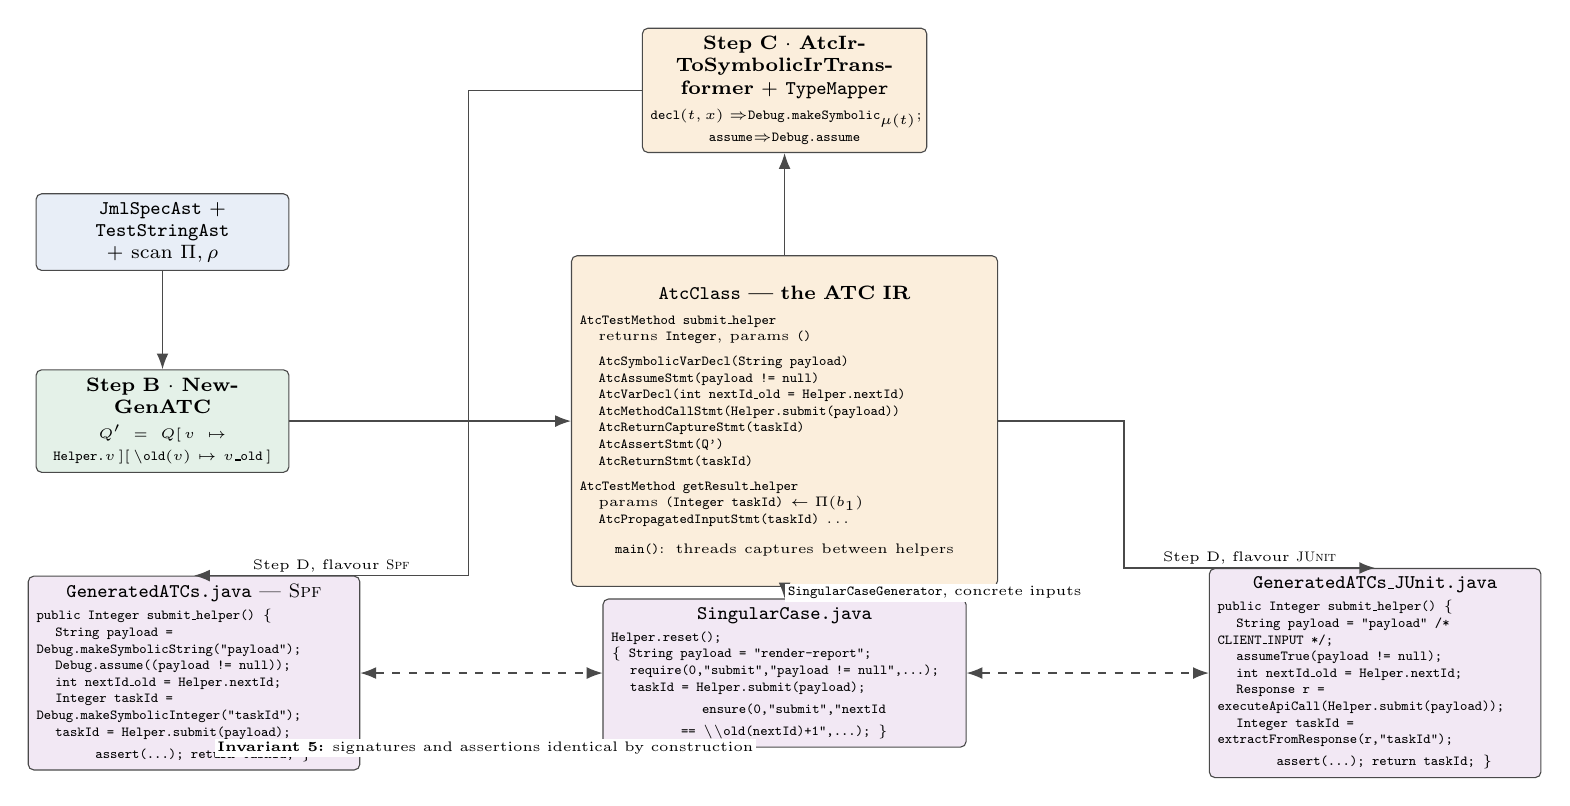
\begin{tikzpicture}
      % ---- the single IR in the centre ----
      \node[corb, text width=52mm, minimum height=42mm] (ir) at (10.5,4.2)
        {\textbf{\texttt{AtcClass} --- the ATC IR}\\[3pt]
         \tiny\raggedright
         \texttt{AtcTestMethod submit\_helper}\\
         \quad returns \texttt{Integer}, params \texttt{()}\\[3pt]
         \quad\texttt{AtcSymbolicVarDecl(String payload)}\\
         \quad\texttt{AtcAssumeStmt(payload != null)}\\
         \quad\texttt{AtcVarDecl(int nextId\_old = Helper.nextId)}\\
         \quad\texttt{AtcMethodCallStmt(Helper.submit(payload))}\\
         \quad\texttt{AtcReturnCaptureStmt(taskId)}\\
         \quad\texttt{AtcAssertStmt(Q')}\\
         \quad\texttt{AtcReturnStmt(taskId)}\\[3pt]
         \texttt{AtcTestMethod getResult\_helper}\\
         \quad params \texttt{(Integer taskId)} $\leftarrow \Pi(b_1)$\\
         \quad\texttt{AtcPropagatedInputStmt(taskId)} \dots\\[3pt]
         \texttt{main()}: threads captures between helpers};

      \node[parb, text width=30mm] (sb) at (2.6,4.2)
        {\textbf{Step B $\cdot$ NewGenATC}\\[1pt]\tiny
         $Q'=Q[\,v\mapsto\texttt{Helper.}v\,][\,\texttt{\textbackslash old}(v)\mapsto v\_\texttt{old}\,]$};
      \node[inb, text width=30mm] (in) at (2.6,6.6)
        {\texttt{JmlSpecAst} $+$ \texttt{TestStringAst} $+$ scan $\Pi,\rho$};
      \draw[fl] (in) -- (sb);
      \draw[fl] (sb) -- (ir);

      % ---- left branch: symbolic ----
      \node[corb, text width=34mm] (sc) at (10.5,8.4)
        {\textbf{Step C $\cdot$ AtcIrToSymbolicIrTransformer} $+$ \texttt{TypeMapper}\\[1pt]\tiny
         \texttt{decl}$(t,x)\Rightarrow$\texttt{Debug.makeSymbolic}$_{\mu(t)}$;\ \ \texttt{assume}$\Rightarrow$\texttt{Debug.assume}};
      \node[outb, text width=40mm] (spf) at (3.0,1.0)
        {\texttt{GeneratedATCs.java} --- \textsc{Spf}\\[2pt]\tiny\raggedright
         \texttt{public Integer submit\_helper() \{}\\
         \quad\texttt{String payload = Debug.makeSymbolicString("payload");}\\
         \quad\texttt{Debug.assume((payload != null));}\\
         \quad\texttt{int nextId\_old = Helper.nextId;}\\
         \quad\texttt{Integer taskId = Debug.makeSymbolicInteger("taskId");}\\
         \quad\texttt{taskId = Helper.submit(payload);}\\
         \quad\texttt{assert(...); return taskId; \}}};

      % ---- right branch: junit ----
      \node[outb, text width=40mm] (ju) at (18.0,1.0)
        {\texttt{GeneratedATCs\_JUnit.java}\\[2pt]\tiny\raggedright
         \texttt{public Integer submit\_helper() \{}\\
         \quad\texttt{String payload = "payload" /* CLIENT\_INPUT */;}\\
         \quad\texttt{assumeTrue(payload != null);}\\
         \quad\texttt{int nextId\_old = Helper.nextId;}\\
         \quad\texttt{Response r = executeApiCall(Helper.submit(payload));}\\
         \quad\texttt{Integer taskId = extractFromResponse(r,"taskId");}\\
         \quad\texttt{assert(...); return taskId; \}}};

      % ---- bottom: singular case ----
      \node[outb, text width=44mm] (sing) at (10.5,1.0)
        {\texttt{SingularCase.java}\\[2pt]\tiny\raggedright
         \texttt{Helper.reset();}\\
         \texttt{\{ String payload = "render-report";}\\
         \quad\texttt{require(0,"submit","payload != null",...);}\\
         \quad\texttt{taskId = Helper.submit(payload);}\\
         \quad\texttt{ensure(0,"submit","nextId == \textbackslash\textbackslash old(nextId)+1",...); \}}};

      \draw[fl] (ir.north) -- (sc.south);
      \draw[fl] (sc.west) -- ++(-2.2,0) |- node[lab, pos=0.75, above] {Step D, flavour \textsc{Spf}} (spf.north);
      \draw[fl] (ir.east) -- ++(1.6,0) |- node[lab, pos=0.75, above] {Step D, flavour \textsc{JUnit}} (ju.north);
      \draw[fl] (ir.south) -- node[lab, right] {\texttt{SingularCaseGenerator}, concrete inputs} (sing.north);
      \draw[{Latex[length=2mm]}-{Latex[length=2mm]}, dashed, draw=cLine] (spf.east) -- (sing.west);
      \draw[{Latex[length=2mm]}-{Latex[length=2mm]}, dashed, draw=cLine] (sing.east) -- (ju.west);
      \node[lab, below=1pt] at (6.7,0.2) {\textbf{Invariant 5:} signatures and assertions identical by construction};
    \end{tikzpicture}}
    \caption{One intermediate representation, three emissions (goal G1), shown on the
    \texttt{taskqueue} example whose test string is \texttt{submit} $\rightarrow$
    \texttt{getResult} $\rightarrow$ \texttt{cancelTask}. The \textsc{Spf} flavour is
    printed from the symbolic IR, the \textsc{JUnit} flavour from the ATC IR directly
    --- which is what lets it see the capture node and emit runtime binding instead of a
    discarded placeholder --- and the singular case from the ATC IR with the concrete
    bindings of the test string. Only the mechanism for obtaining a
    \textsc{Server\_Output} differs between the two flavours; the method signatures
    and the assertions are the same text.}
    \label{fig:dual}
\end{figure*}

\subsection{Step B: Building the ATC IR}

For each block, \texttt{NewGenATC} emits an ordered helper body
\begin{equation}
\mathcal{B}(b_i)=\big\langle\,
\mathrm{assume}(P_{f_i}),\
\mathrm{snap}(\mathcal{O}(Q_{f_i})),\
\mathrm{call},\
\mathrm{capture},\
\mathrm{assert}(Q'_{f_i})
\,\big\rangle
\end{equation}
where $\mathcal{O}(Q)$ is the set of names appearing under
\texttt{\textbackslash old} in $Q$, and the postcondition is rewritten by two
substitutions applied in order,
\begin{equation}
Q' \;=\; Q\big[\,v\mapsto\texttt{Helper.}v\,\big]_{v\in V}
         \big[\,\texttt{\textbackslash old}(v)\mapsto v\_\texttt{old}\,\big]_{v\in\mathcal{O}(Q)} .
\end{equation}
The order matters: state names are qualified first so that a snapshot local, which
is an ordinary Java local and not library state, is not qualified with it. The
choice between the library path above and the older functional path is made on
whether $V=\varnothing$, not on whether the sequence handles return values ---
a distinction established in Section~\ref{sec:eval} as one of four defects that
generated sequences exposed.

\subsection{Step C: Symbolic Transformation}

Step~C rewrites the IR node by node for Symbolic PathFinder. With $\mu$ the type map
carried by \texttt{TypeMapper},
\begin{equation}
\mathcal{T}\big(\mathrm{decl}(t,x)\big)=
\big[\,x \leftarrow \texttt{Debug.makeSymbolic}_{\mu(t)}(\text{``}x\text{''})\,\big]
\end{equation}
\begin{equation}
\mathcal{T}\big(\mathrm{assume}(c)\big)=\texttt{Debug.assume}(c),\qquad
\mathcal{T}\big(\mathrm{assert}(c)\big)=\mathrm{assert}(c).
\end{equation}
$\mu$ routes primitives and boxed primitives to the primitive factories
(\texttt{Integer} to \texttt{makeSymbolicInteger}, \texttt{double} to
\texttt{makeSymbolicReal}), collections to concrete initialisation, and anything
else to a symbolic reference --- a fallback that, across the fourteen registered
libraries, is never taken.

\subsection{Step D: Dual-Flavour Emission}

Step~D visits an IR and prints Java under one of two flavours. The architectural
point is what the two share. Writing $\mathcal{G}_{\textsc{spf}}$ and
$\mathcal{G}_{\textsc{junit}}$ for the two emissions of one \texttt{AtcClass} $K$,
and $\mathrm{sig}$ and $\mathrm{asrt}$ for the sequences of helper signatures and
assertion texts in a file,
\begin{equation}
\mathrm{sig}\big(\mathcal{G}_{\textsc{spf}}(K)\big)=\mathrm{sig}\big(\mathcal{G}_{\textsc{junit}}(K)\big)
\ \wedge\
\mathrm{asrt}\big(\mathcal{G}_{\textsc{spf}}(K)\big)=\mathrm{asrt}\big(\mathcal{G}_{\textsc{junit}}(K)\big).
\end{equation}
Only the mechanism for obtaining a \textsc{Server\_Output} differs: a symbolic
placeholder the solver reasons about, or an \texttt{executeApiCall} /
\texttt{extractFromResponse} pair that reads the real value back at runtime.
Fig.~\ref{fig:dual} shows both, side by side, on the same helper.

A second decision is forced by this sharing. Step~C wants a fresh symbolic variable
in every consuming block; Step~D wants a propagated value to be a formal parameter
threaded from \texttt{main}. Both hold at once by making the parameter real and
re-binding it symbolically \emph{in the \textsc{Spf} body only}: cross-block equality
then reaches the solver as a constraint rather than as an assignment, while the
\textsc{JUnit} body simply uses the argument it was given.

\subsection{Algorithms}

\begin{algorithm}[H]
\caption{Step A --- the propagation scan}
\begin{algorithmic}[1]
\REQUIRE specification $\Sigma=\langle V,F\rangle$; test string $\tau=\langle b_0,\dots,b_{n-1}\rangle$
\ENSURE per-block trace, $\Pi(f)$ for every $f$, producer and type maps
\FOR{$i = 0$ to $n-1$}
    \STATE $f \leftarrow f_i$;\ \ $\Pi_i \leftarrow \varnothing$
    \STATE \textbf{for each} $p \in \mathit{params}(f)$: \textbf{if} $\mathit{name}(p)\in A$ \textbf{then} $\Pi_i \leftarrow \Pi_i\cup\{p\}$, mark $p$ as \textsc{Server\_Output}; \textbf{else} warn if $\mathit{type}(p)$ matches some $a\in A$
    \STATE $\Pi(f) \leftarrow \Pi(f)\cup\Pi_i$
    \STATE $r \leftarrow \rho(f)$ \COMMENT{the \texttt{\textbackslash result} binding, or none}
    \STATE \textbf{if} $r \neq \bot$ \textbf{then} $A \leftarrow A\cup\{r\}$; $\mathit{producer}[r]\leftarrow f$; $\mathit{type}[r]\leftarrow$ return type of $f$
    \STATE append $\langle i,f,\Pi_i,r,A\rangle$ to the trace
\ENDFOR
\STATE $A \leftarrow \varnothing$ initially; each $r$ enters $A$ only after its own block
\RETURN trace, $\Pi$, $\mathit{producer}$, $\mathit{type}$
\end{algorithmic}
\end{algorithm}

\begin{algorithm}[H]
\caption{Mutation evaluation of a generated suite}
\begin{algorithmic}[1]
\REQUIRE library key $k$; mutation set $M_k$; specification and test string of $k$
\ENSURE a verdict per mutant and the mutation score $\mathit{MS}_k$
\STATE $\mathit{killed}\leftarrow 0$;\ \ $\mathit{survived}\leftarrow 0$;\ \ $\mathit{invalid}\leftarrow 0$
\FOR{each mutant $m \in M_k$}
    \STATE copy every source of $k$ into a private sandbox and rewrite the single line $m.\mathit{find}$ inside method $m.\mathit{in}$ of file $m.\mathit{file}$
\ENDFOR
\STATE regenerate nothing in advance --- no result is reused between mutants
\FOR{each sandboxed mutant $m$}
    \IF{the line matched exactly once \textbf{and} the sandbox compiles}
        \STATE re-run the whole pipeline: parse $\Sigma$ and $\tau$, Step~A--D, emit, \texttt{javac}, fork \texttt{SingularCase} and the \textsc{JUnit} flavour under a watchdog
    \ELSE
        \STATE $\mathit{invalid}\leftarrow \mathit{invalid}+1$;\ \textbf{continue}
    \ENDIF
    \STATE classify: some generated condition rejected $m$ or the run timed out $\Rightarrow$ \textsc{Killed}; every condition still held $\Rightarrow$ \textsc{Survived}; compare against $m.\mathit{expect}$
\ENDFOR
\STATE $\mathit{MS}_k \leftarrow \mathit{killed}/(\mathit{killed}+\mathit{survived})$ \COMMENT{invalid mutants measure nothing and are excluded}
\RETURN verdicts, $\mathit{MS}_k$, and the per-operator breakdown
\end{algorithmic}
\end{algorithm}

\section{Architectural Invariants}
\label{sec:invariants}

\subsection{Why Invariants Rather Than Tests}

A generator has two failure modes, and only one of them is a wrong answer. The other
is a right answer produced by accident --- a helper that happens to have the correct
signature because the example is small, a flavour that happens to agree because
nothing in it was exercised. Behavioural tests cannot separate the two. The suite
therefore contains two distinct test classes: one asserts on the \emph{behaviour} of
generated code (every condition of every singular case, as an individually named
JUnit test), and one asserts on the generated \emph{text} --- propagation traces,
helper signatures, the absence of particular tokens, and a comparison against
reviewed golden copies. The second class walks the example registry, so a newly
added library is held to every invariant below at once.

\subsection{The Seven Cross-Example Invariants}

\textbf{Invariant 1 (empty parameter lists).} An operation that takes no arguments
and returns a value is emitted with an empty formal parameter list, never with its
own return threaded into it:
\begin{equation}
\mathit{params}(f)=\varnothing \;\Rightarrow\; \mathrm{sig}(f\_\mathit{helper})=\tau_f\ f\_\mathit{helper}()
\end{equation}

\textit{Proof Sketch:} A helper's parameter list is exactly $\Pi(f)$, and by
construction $\Pi(f)\subseteq\mathit{params}(f)$, since the scan only ever marks an
existing formal parameter as propagated. With $\mathit{params}(f)=\varnothing$ the
list is empty regardless of $A$. The same containment gives the stronger statement
checked over the whole registry,
\begin{equation}
\forall m\in\mathcal{H}\ \ \forall p\in\mathit{params}(m):\ p\in\Pi(f_m),
\end{equation}
that is, no helper anywhere carries a parameter the scan did not mark.

\textbf{Invariant 2 (nullable outputs attract no assertion).} A
\textsc{Server\_Output} that the specification constrains nowhere must appear in no
generated assertion:
\begin{equation}
x\notin \mathrm{Vars}(Q_f)\ \ \forall f \;\Rightarrow\; x\notin\bigcup\nolimits_{a\in\mathrm{asrt}}\mathrm{Vars}(a)
\end{equation}
The \texttt{hashmap} example exists to exercise this: \texttt{put} returns the
previous value, which is \texttt{null} when the key was absent, and the
specification deliberately says nothing about it. The invariant forbids the
generator from inventing a non-null check that the contract does not license --- and
the surviving mutant \texttt{HASHMAP\_PUT\_OLDVAL\_FABRICATED} is the evidence that
it holds.

\textbf{Invariant 3 (produced but unconsumed).} A captured value with no downstream
consumer stays valid: it is captured, returned by its helper, and forced into no
parameter list.

\textbf{Invariant 4 (multi-hop propagation).} One value threads through arbitrarily
many consuming blocks, with the return type of each helper unaffected:
\begin{equation}
r\in A_i \wedge r\in A_j,\ i<j \;\Rightarrow\; r\in\mathit{params}(f_i\_\mathit{helper})\cap\mathit{params}(f_j\_\mathit{helper})
\end{equation}

\textbf{Invariant 5 (flavour agreement).} Equation~(7): the two flavours share their
signatures and assertions verbatim, and differ in exactly the documented way --- the
\textsc{JUnit} file contains no \texttt{Debug.} token at all, and for every
\textsc{Server\_Output} it contains the matching \texttt{executeApiCall} and
\texttt{extractFromResponse} pair.

\textbf{Invariant 6 (snapshots are ordinary locals).} An \texttt{\textbackslash old}
snapshot is a plain read of the declared state type, never a symbolic value and never
a special-cased node. This is what allows the same snapshot text to appear unchanged
in all three emissions.

\textbf{Invariant 7 (boxed primitives).} A boxed \textsc{Server\_Output} routes to the
primitive symbolic factory, so that \texttt{Integer} stays boxed --- keeping
\texttt{null} representable --- while still being solvable; the
\texttt{makeSymbolicRef} fallback is reached by none of the registered libraries.

\section{Evaluation}
\label{sec:eval}

\subsection{Hand-Written Mutation Sets}

Each library carries a set of single-line faults, each declaring a mutation operator,
the method to search, the line to replace, and an \emph{expectation}:
\texttt{expect: killed} by default, or \texttt{expect: survives} with a mandatory
\texttt{note} saying why. A survivor nobody explained is indistinguishable from a gap
nobody noticed, so the parser rejects one without a note. Declaring the expectation
turns the file into a two-way regression check: tighten a postcondition and a declared
survivor starts dying, failing the test until the improvement is recorded; weaken one
and a mutant that used to die starts surviving, so the regression cannot pass quietly.
Table~\ref{tab:perlib} gives the per-library result of the last recorded full run.

\begin{table}[h]
\centering
\caption{Hand-written mutation sets, per library. Invalid mutants were zero throughout
and are excluded from the score, $\mathit{MS}=\mathit{killed}/(\mathit{killed}+\mathit{survived})$.}
\label{tab:perlib}
\begin{tabular}{|l|c|c|c|}
\hline
\textbf{Library} & \textbf{Mutants} & \textbf{Killed} & \textbf{Score} \\
\hline
arraylib & 9 & 7 & 77.8\% \\
\hline
bst & 8 & 7 & 87.5\% \\
\hline
graph & 8 & 6 & 75.0\% \\
\hline
hashmap & 11 & 9 & 81.8\% \\
\hline
heap & 9 & 8 & 88.9\% \\
\hline
linkedlist & 7 & 5 & 71.4\% \\
\hline
lrucache & 8 & 7 & 87.5\% \\
\hline
mathlib & 12 & 8 & 66.7\% \\
\hline
orderservice & 14 & 12 & 85.7\% \\
\hline
queue & 8 & 7 & 87.5\% \\
\hline
set & 6 & 4 & 66.7\% \\
\hline
stack & 11 & 8 & 72.7\% \\
\hline
taskqueue & 11 & 8 & 72.7\% \\
\hline
ticketservice & 13 & 11 & 84.6\% \\
\hline
\textbf{ALL} & \textbf{135} & \textbf{107} & \textbf{79.3\%} \\
\hline
\end{tabular}
\end{table}

The twenty-eight survivors sort into four groups, and the group is the finding rather
than the percentage. Seven survive because \emph{the test string never asks}: the
single checked-in sequence is too short or too uniform to separate the fault from
correct behaviour, and each dies against a longer sequence with no change to any
specification. Six survive because \emph{the specification could say it and does not};
the clearest pair in the set is \texttt{STACK\_POP\_FROM\_BOTTOM}, which survives
because \texttt{Stack.spec} never names which element \texttt{pop} returned, beside the
identical fault in \texttt{queue}, which dies because \texttt{Queue.spec} writes
\texttt{dequeuedElem == \textbackslash old(head)}. Seven survive because \emph{the
grammar cannot say it at all} --- they need a summing quantifier, a conditional
expression, or a way to name an individual element. And one,
\texttt{BST\_INSERT\_TIES\_GO\_LEFT}, is \emph{unreachable rather than undetected}: the
precondition of \texttt{insert} requires the key to be absent, which is the price paid
for an unconditional \texttt{size == \textbackslash old(size) + 1}. A stronger
precondition always buys a stronger postcondition with exactly this currency.

\subsection{Generated Suites and the Per-Operator Score}

A single percentage is a poor summary, so every mutant declares which \emph{kind} of
fault it is, from a closed vocabulary of seventeen operators following the classical
Mothra set. The vocabulary is enforced by the parser, which is what makes the
per-operator column a measurement rather than a tally of whatever words people wrote.
Table~\ref{tab:ops} gives the breakdown, beside the mechanically generated suite of
Fig.~\ref{fig:suites}.

\begin{table*}[t]
\centering
\caption{Mutation score by operator. \textit{Hand-written} covers the 135 declared
faults of Table~\ref{tab:perlib} across all fourteen libraries. \textit{Generated}
covers the mechanically produced suite for \texttt{stack} --- every operator applied to
every admitting line --- scored first against the single checked-in test string
(\textit{alone}) and then against the generated family of 260 sequences
(\textit{family}). A dash means the suite contains no mutant of that operator;
\texttt{VRO} was added for the generated suites and its two hand-written mutants
postdate the recorded run.}
\label{tab:ops}
\setlength{\tabcolsep}{3pt}
\scriptsize
\begin{tabular}{|l|c|c|c|c|c|c|c|c|c|c|c|}
\hline
 & & \multicolumn{4}{c|}{\textbf{Hand-written (14 libraries)}} & \multicolumn{6}{c|}{\textbf{Generated (\texttt{stack})}} \\
\hline
\textbf{Operator} & \textbf{Abbr} & \textbf{Mut.} & \textbf{Killed} & \textbf{Surv.} & \textbf{Score} & \textbf{Mut.} & \textbf{Killed} & \textbf{Surv.} & \textbf{Inv.} & \textbf{Alone} & \textbf{Family} \\
\hline
arithmetic-operator-replacement & AOR & 6 & 5 & 1 & 83.3\% & 12 & 9 & 3 & 0 & 75.0\% & 91.7\% \\
\hline
arithmetic-operator-insertion & AOI & 7 & 5 & 2 & 71.4\% & 2 & 2 & 0 & 0 & 100.0\% & 100.0\% \\
\hline
relational-operator-replacement & ROR & 5 & 2 & 3 & 40.0\% & --- & --- & --- & --- & --- & --- \\
\hline
conditional-operator-replacement & COR & 2 & 2 & 0 & 100.0\% & --- & --- & --- & --- & --- & --- \\
\hline
conditional-operator-insertion & COI & 4 & 2 & 2 & 50.0\% & --- & --- & --- & --- & --- & --- \\
\hline
unary-operator-insertion & UOI & 7 & 6 & 1 & 85.7\% & 1 & 1 & 0 & 0 & 100.0\% & 100.0\% \\
\hline
absolute-value-insertion & ABS & 2 & 2 & 0 & 100.0\% & 1 & 1 & 0 & 0 & 100.0\% & 100.0\% \\
\hline
constant-replacement & CRP & 7 & 6 & 1 & 85.7\% & 11 & 10 & 1 & 0 & 90.9\% & 100.0\% \\
\hline
condition-to-constant & CTC & 2 & 2 & 0 & 100.0\% & --- & --- & --- & --- & --- & --- \\
\hline
loop-bound-replacement & LBR & 4 & 1 & 3 & 25.0\% & --- & --- & --- & --- & --- & --- \\
\hline
return-value-replacement & RVR & 14 & 9 & 5 & 64.3\% & 2 & 1 & 1 & 0 & 50.0\% & 50.0\% \\
\hline
statement-deletion & SDL & 41 & 40 & 1 & 97.6\% & 5 & 4 & 0 & 1 & 100.0\% & 100.0\% \\
\hline
statement-replacement & STR & 6 & 5 & 1 & 83.3\% & 1 & 1 & 0 & 0 & 100.0\% & 100.0\% \\
\hline
argument-replacement & ARP & 13 & 7 & 6 & 53.8\% & 2 & 0 & 1 & 1 & 0.0\% & 100.0\% \\
\hline
method-call-replacement & MCR & 5 & 3 & 2 & 60.0\% & 9 & 7 & 2 & 0 & 77.8\% & 100.0\% \\
\hline
side-effect-insertion & SEI & 10 & 10 & 0 & 100.0\% & 5 & 3 & 1 & 1 & 75.0\% & 75.0\% \\
\hline
variable-replacement & VRO & 2 & --- & --- & --- & --- & --- & --- & --- & --- & --- \\
\hline
\textbf{ALL} & & \textbf{135} & \textbf{107} & \textbf{28} & \textbf{79.3\%} & \textbf{51} & \textbf{39} & \textbf{9} & \textbf{3} & \textbf{81.3\%} & \textbf{93.8\%} \\
\hline
\end{tabular}
\end{table*}

Read down the hand-written score column and the clauses sort themselves into two
kinds. The operators that change \emph{how much work happens} are caught almost
always --- \texttt{SDL} at 97.6\% and \texttt{SEI} at 100\% --- because nearly every
specification in the set counts something (\texttt{size}, \texttt{writes},
\texttt{events}, \texttt{edgeCount}, \texttt{nextId}), and a counter is exactly what an
\texttt{\textbackslash old} clause compares. The operators that change \emph{which
value comes back} are missed most often --- \texttt{LBR} at 25\%, \texttt{ROR} at 40\%,
\texttt{ARP} at 53.8\% --- and they fail together for one reason: a loop one iteration
short still returns \emph{a} number, a flipped comparison still returns \emph{an} index,
and the specifications constrain the \emph{range} of an answer
($\texttt{total} \geq 0$, $-1 \leq \texttt{position} < \texttt{size}$) because the
grammar has no quantifier with which to constrain its \emph{value}. That is one
finding, not fifteen: \textbf{this pipeline is good at catching faults in bookkeeping
and bad at catching faults in answers, and the cause is a missing quantifier rather
than a missing test.} It also explains why \texttt{RVR} sits in the middle at 64\%: a
returned value that is \emph{state-bearing} (a hold identifier, an evicted key) is
caught by the state clauses around it, and one that is merely \emph{computed} is not.

The right-hand half of Table~\ref{tab:ops} measures the claim the survivor notes keep
making. Several notes assert that a fault would die against a longer sequence with no
change to the specification --- a claim about the test string, asserted by the same
person who wrote the sequence that failed to catch the fault. Fig.~\ref{fig:suites}
turns it into a measurement: for \texttt{stack}, six of the nine survivors die against
the generated family, lifting the score from 81.3\% to 93.8\%. The difference between
those two numbers is the part of the score that was never about the specification at
all.

Generating suites also tests the pipeline, and four defects surfaced that no
hand-written test string could reach. A whole code path was selected by the wrong
question (the library path was chosen on \emph{does anything here return a value?}
rather than \emph{does the specification declare state?}, and every checked-in sequence
happened to answer both the same way). A \textsc{Client\_Input} could collide with a
capture when a consumer preceded its producer. \texttt{main} could pass a value four
blocks before it existed, because a helper's parameter list is per \emph{function}
while propagation is per \emph{block}. And the harness could hang forever, since moving
a loop bound is precisely how a loop stops terminating --- there is now a ten-second
watchdog, and a mutant that reaches it is counted as killed, which is what
\textsc{Timed\_Out} means in the literature.

\begin{figure}[H]
\centering
\resizebox{\linewidth}{!}{%
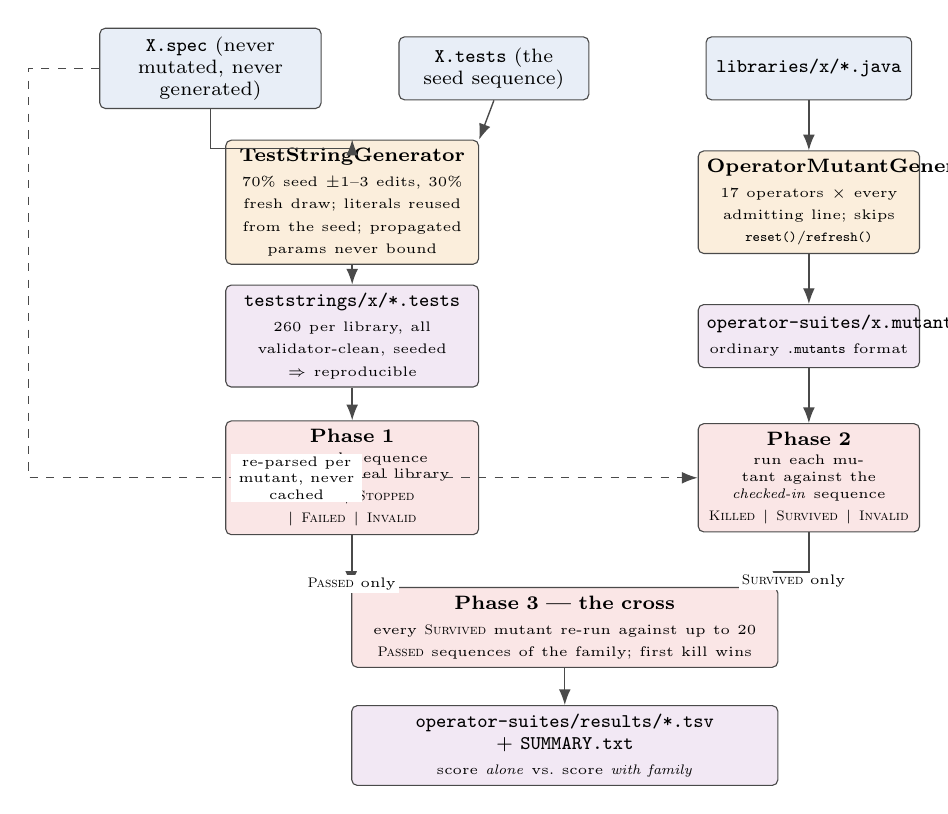
\begin{tikzpicture}
  \node[inb, text width=26mm] (spec) at (0,8.6) {\texttt{X.spec} (never mutated, never generated)};
  \node[inb, text width=22mm] (seed) at (3.6,8.6) {\texttt{X.tests} (the seed sequence)};
  \node[inb, text width=24mm] (src)  at (7.6,8.6) {\texttt{libraries/x/*.java}};

  \node[corb, text width=30mm] (tsg) at (1.8,6.9) {\textbf{TestStringGenerator}\\[1pt]\tiny 70\% seed $\pm$1--3 edits, 30\% fresh draw; literals reused from the seed; propagated params never bound};
  \node[corb, text width=26mm] (omg) at (7.6,6.9) {\textbf{OperatorMutantGenerator}\\[1pt]\tiny 17 operators $\times$ every admitting line; skips \texttt{reset()}/\texttt{refresh()}};

  \node[outb, text width=30mm] (fam) at (1.8,5.2) {\texttt{teststrings/x/*.tests}\\[1pt]\tiny 260 per library, all validator-clean, seeded $\Rightarrow$ reproducible};
  \node[outb, text width=26mm] (mut) at (7.6,5.2) {\texttt{operator-suites/x.mutants}\\[1pt]\tiny ordinary \texttt{.mutants} format};

  \node[evab, text width=30mm] (p1) at (1.8,3.4) {\textbf{Phase 1}\\[1pt]\tiny run each sequence against the real library\\ \textsc{Passed} $\mid$ \textsc{Stopped} $\mid$ \textsc{Failed} $\mid$ \textsc{Invalid}};
  \node[evab, text width=26mm] (p2) at (7.6,3.4) {\textbf{Phase 2}\\[1pt]\tiny run each mutant against the \emph{checked-in} sequence\\ \textsc{Killed} $\mid$ \textsc{Survived} $\mid$ \textsc{Invalid}};

  \node[evab, text width=52mm] (p3) at (4.5,1.5) {\textbf{Phase 3 --- the cross}\\[1pt]\tiny every \textsc{Survived} mutant re-run against up to 20 \textsc{Passed} sequences of the family; first kill wins};
  \node[outb, text width=52mm] (res) at (4.5,0.0) {\texttt{operator-suites/results/*.tsv} $+$ \texttt{SUMMARY.txt}\\[1pt]\tiny score \emph{alone} vs.\ score \emph{with family}};

  \draw[fl] (spec.south) -- ++(0,-0.5) -| (tsg.north);
  \draw[fl] (seed.south) -- (tsg.north east);
  \draw[fl] (src.south)  -- (omg.north);
  \draw[fl] (tsg) -- (fam);
  \draw[fl] (omg) -- (mut);
  \draw[fl] (fam) -- (p1);
  \draw[fl] (mut) -- (p2);
  \draw[fl] (p1.south) -- ++(0,-0.5) -| node[lab, pos=0.25, below] {\textsc{Passed} only} (p3.north west);
  \draw[fl] (p2.south) -- ++(0,-0.5) -| node[lab, pos=0.25, below] {\textsc{Survived} only} (p3.north east);
  \draw[fl] (p3) -- (res);
  \draw[flb] (spec.west) -- ++(-0.9,0) |- node[lab, pos=0.75, left] {\parbox{16mm}{\centering re-parsed per mutant, never cached}} (p2.west);
\end{tikzpicture}}
\caption{The generated-suite architecture. The specification is the fixed point of the
exercise: what varies is the sequence the library is exercised with (Phase 1) and the
library itself (Phase 2). Phase 3 is the only phase that uses both halves, and it is
what the other two exist for.}
\label{fig:suites}
\end{figure}

\section{Conclusion and Future Work}

We have described an architecture in which a behavioural contract and an explicit call
sequence are compiled, through one intermediate representation, into three executable
test artefacts whose signatures and assertions cannot disagree. The organising
distinction is between values the caller invents and values the library invents, and
the propagation scan that enforces it is a small analysis with large architectural
consequences: it determines helper signatures, what \texttt{main} threads where, what
the validator may reject, and what a generated test string is forbidden to bind. Seven
invariants over the generated \emph{text}, checked against reviewed golden copies for
every registered library, are what keep the property true as the system grows.

Mutation testing grades the specifications rather than the generator, and its
per-operator breakdown gives a sharper instruction than any aggregate score could: the
contracts are strong about bookkeeping and weak about answers. The three directions
that follow are therefore concrete. First, \textbf{quantifiers} --- a summing quantifier
and a bounded universal would directly address \texttt{LBR}, \texttt{ROR} and the
\texttt{ARP} survivors, which are the same failure wearing three names. Second,
\textbf{conditional postconditions}, whose absence is why \texttt{HashMapLib.spec} omits
the size clause that holds only when a key was absent, and why \texttt{indexOf} can only
be constrained by its range. Third, \textbf{structural propagation}: matching is by name
today, and a type-directed or alias-directed match would remove the one place where the
system degrades to a warning. Beyond the language, the generated-suite run is currently
complete for one library and partial for the rest, and equivalent-mutant detection
remains the standard open problem --- which is why the generated score is reported
beside the hand-written one rather than instead of it.

\begin{thebibliography}{00}
\bibitem{b1} G. T. Leavens, A. L. Baker, and C. Ruby, ``Preliminary design of JML: a behavioral interface specification language for Java,'' \textit{ACM SIGSOFT Software Engineering Notes}, vol. 31, no. 3, pp. 1--38, 2006.
\bibitem{b2} W. Visser, K. Havelund, G. Brat, S. Park, and F. Lerda, ``Model checking programs,'' \textit{Automated Software Engineering}, vol. 10, no. 2, pp. 203--232, 2003.
\bibitem{b3} C. S. P\u{a}s\u{a}reanu, W. Visser, D. Bushnell, J. Geldenhuys, P. Mehlitz, and N. Rungta, ``Symbolic PathFinder: integrating symbolic execution with model checking for Java bytecode analysis,'' \textit{Automated Software Engineering}, vol. 20, no. 3, pp. 391--425, 2013.
\bibitem{b4} R. A. DeMillo, R. J. Lipton, and F. G. Sayward, ``Hints on test data selection: help for the practicing programmer,'' \textit{Computer}, vol. 11, no. 4, pp. 34--41, 1978.
\bibitem{b5} Y. Jia and M. Harman, ``An analysis and survey of the development of mutation testing,'' \textit{IEEE Transactions on Software Engineering}, vol. 37, no. 5, pp. 649--678, 2011.
\end{thebibliography}

\end{document}
